\begin{center}
	\begin{tabular}{M{6.5cm}M{11cm}}
		\textbf{TRUNG TÂM MANABIE}& \textbf{ĐỀ ÔN TẬP KIỂM TRA GIỮA HỌC KÌ 1}\\
		\textbf{MÃ ĐỀ: 002}& \textbf{Bài thi môn: VẬT LÝ 11}\\
		\textit{(Đề thi có 05 trang)}& \textit{Thời gian làm bài: 50 phút, không kể thời gian phát đề}
		
		\noindent\rule{4cm}{0.8pt} \\
	\end{tabular}
\end{center}
\setcounter{section}{0}
\section{Câu trắc nghiệm nhiều phương án lựa chọn}
\textit{Thí sinh trả lời từ câu 1 đến câu 18. Mỗi câu hỏi thí sinh chọn một phương án}
\setcounter{ex}{0}
\Opensolutionfile{ans}[ans/G11-4-TN]
% ===================================================================
\begin{ex}
	Một vật dao động điều hòa trên trục $Ox$. Vận tốc của vật
	\choice
	{\True biến thiên điều hòa theo thời gian}
	{là hàm bậc hai của thời gian}
	{luôn có giá trị không đổi}
	{luôn có giá trị dương}
	\loigiai{}
\end{ex}
% ===================================================================
\begin{ex}
	Một vật dao động điều hòa có phương trình li độ $x=\xsi{12\cos\left(4\pi t\right)}{\centi\meter}$. Biên độ dao động của vật là	
	\choice
	{\True $A=\SI{6}{\centi\meter}$}
	{$A=\SI{12}{\centi\meter}$}
	{$A=\xsi{4\pi}{\centi\meter}$}
	{$A=\SI{4}{\centi\meter}$}
	\loigiai{}
\end{ex}
% ===================================================================
\begin{ex}
	Tốc độ cực đại của dao động điều hòa có biên độ $A$ và tần số $\gamma$ là 
	\choice
	{$\gamma A^2$}
	{$2\pi\gamma A^2$}
	{$\gamma A$}
	{\True $2\pi\gamma A$}
	\loigiai{}
\end{ex}
% ===================================================================
\begin{ex}
	Một vật nhỏ khối lượng $m$, dao động điều hòa với phương trình li độ $x=A\cos\left(\omega t+\varphi\right)$ với $A$, $\omega$, $\varphi$ là các hằng số. Cơ năng của vật là
	\choice
	{$\dfrac{1}{2}m\omega A^2$}
	{$m\omega A^2$}
	{\True $\dfrac{1}{2}m\omega^2 A^2$}
	{$\dfrac{1}{2}m\omega^2 A$}
	\loigiai{}
\end{ex}
% ===================================================================
\begin{ex}
	Một vật dao động điều hòa có phương trình $x=A\cos\left(\omega t-\dfrac{\pi}{3}\right)$. Gốc thời gian $t = 0$ đã được chọn khi vật qua li độ 
	\choice
	{$x=\dfrac{A}{2}$ theo chiều âm quĩ đạo}
	{\True $x=\dfrac{A}{2}$ theo chiều dương quĩ đạo}
	{$x=\dfrac{A\sqrt{3}}{2}$ theo chiều âm quĩ đạo}
	{$x=\dfrac{A\sqrt{3}}{2}$ theo chiều dương quĩ đạo}
	\loigiai{}
\end{ex}
% ===================================================================
\begin{ex}
	Một vật nhỏ dao động điều hòa trên trục $Ox$ có phương trình li độ $x=A\cos\left(\omega t+\varphi\right)$. Vận tốc của vật có biểu thức là	
	\choice
	{$v=\omega A\sin\left(\omega t+\varphi\right)$}
	{$v=\omega A\cos\left(\omega t+\varphi\right)$}
	{\True $v=-\omega A\sin\left(\omega t+\varphi\right)$}
	{$v=-\omega A\cos\left(\omega t+\varphi\right)$}
	\loigiai{}
\end{ex}
% ===================================================================
\begin{ex}
	Một vật dao động điều hòa khi đi từ vị trí cân bằng ra biên thì
	\choice
	{cơ năng tăng}
	{động năng tăng thế năng giảm}
	{\True động năng giảm thế năng tăng}
	{cơ năng giảm}
	\loigiai{}
\end{ex}
% ===================================================================
\begin{ex}
Con lắc lò xo gồm vật nặng có khối lượng $m=\SI{0.4}{\kilogram}$, tần số góc $\SI{20}{\radian/\second}$ dao động điều hòa theo phương ngang. Khi ở li độ $\SI{2}{\centi\meter}$ thì vận tốc của vật bằng $\SI{40}{\centi\meter/\second}$. Năng lượng dao động của vật là	
	\choice
	{$\SI{0.032}{\joule}$}
	{$\SI{0.64}{\joule}$}
	{$\SI{1.6}{\joule}$}
	{\True $\SI{0.064}{\joule}$}
	\loigiai{
	$$W=\dfrac{1}{2}m\omega^2x^2+\dfrac{1}{2}mv^2=\SI{0.064}{\joule}.$$
	}
\end{ex}


% ===================================================================
\begin{ex}
	Tại một nơi trên Trái Đất, con lắc đơn có chiều dài $\ell$   dao động điều hòa với chu kì $T$. Nếu chiều dài của con lắc  tăng bốn lần thì chu kì lúc này bằng
	\choice
	{$\sqrt{2}T$}
	{$T$}
	{$4T$}
	{\True $2T$}
	\loigiai{
	$$T\sim\sqrt{\ell}\Rightarrow \dfrac{T'}{T}=\sqrt{\dfrac{\ell'}{\ell}}=2.$$
	}
\end{ex}
% ===================================================================
\begin{ex}
	Một vật dao động điều hòa chuyển động từ vị trí biên về vị trí cân bằng thì
	\choice
	{vận tốc tăng nhanh dần đều}
	{\True vận tốc và lực kéo về cùng dấu}
	{tốc độ của vật giảm dần}
	{gia tốc có độ lớn tăng dần}
	\loigiai{}
\end{ex}
% ===================================================================
\begin{ex}
	Một vật dao động điều hòa có chu kỳ $T$. Thời gian ngắn nhất vật chuyển động từ vị trí biên về vị trí gia tốc có độ lớn bằng một nửa độ lớn cực đại là
	\choice
	{$\dfrac{T}{8}$}
	{$\dfrac{T}{4}$}
	{$\dfrac{T}{12}$}
	{\True $\dfrac{T}{6}$}
	\loigiai{}
\end{ex}
% ===================================================================
\begin{ex}
	Một vật dao động điều hòa có phương trình gia tốc theo li độ là $a =\xsi{-100x}{\centi\meter/\second^2}$. Tần số góc của dao động bằng
	\choice
	{$\SI{50}{\radian/\second}$}
	{$\SI{100}{\radian/\second}$}
	{$\SI{200}{\radian/\second}$}
	{\True $\SI{10}{\radian/\second}$}
	\loigiai{
	$$\omega =\sqrt{-\dfrac{a}{x}}=\SI{10}{\radian/\second}.$$
	}
\end{ex}
% ===================================================================
\begin{ex}
Một vật dao động điều hòa với biên độ $A$ dọc theo trục $Ox$ và quanh gốc tọa độ O. Một đại lượng $Y$ nào đó của vật phụ thuộc vào li độ $x$ của vật của vật theo đồ thị có dạng một phần của đường parabol như hình vẽ bên. $Y$ là đại lượng nào sau đây?	
\begin{center}
	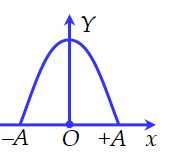
\includegraphics[width=0.2\linewidth]{../figs/D11-004-1}
\end{center}
	\choice
	{Vận tốc}
	{Thế năng}
	{\True Động năng}
	{Gia tốc}
	\loigiai{}
\end{ex}
% ===================================================================
\begin{ex}
	Một chất điểm dao động điều hòa quanh vị trí cân bằng O với chiều dài quỹ đạo là $L=\SI{12}{\centi\meter}$. Hình bên là đồ thị biểu diễn pha dao động ($\alpha_v$) của vận tốc  của chất điểm theo thời gian $t$. Phương trình gia tốc của chất điểm là
	\begin{center}
		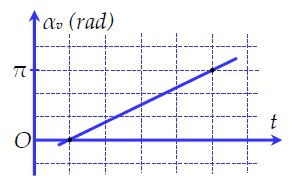
\includegraphics[width=0.35\linewidth]{../figs/D11-004-2}
	\end{center}
	\choice
	{$a=6\omega\cos\left(\omega t+\dfrac{\pi}{4}\right)$}
	{$a=6\omega\cos\left(\omega t-\dfrac{3\pi}{4}\right)$}
	{$a=6\omega^2\cos\left(\omega t-\dfrac{3\pi}{4}\right)$}
	{\True $a=6\omega^2\cos\left(\omega t+\dfrac{\pi}{4}\right)$}
	\loigiai{
	Pha ban đầu của $v$:
	$$\varphi_{0v}=\xsi{-\dfrac{\pi}{4}}{\radian}.$$
	Pha ban đầu của $a$:
	$$\varphi_{0a}=\varphi_{0v}+\dfrac{\pi}{2}=\xsi{\dfrac{\pi}{4}}{\radian}.$$
	}
\end{ex}
% ===================================================================
\begin{ex}
	Một chất điểm dao động điều hòa trên phương nằm ngang có chiều dài quỹ đạo bằng $\SI{24}{\centi\meter}$ và chu kì $T=\SI{0.8}{\second}$. Chọn gốc thời gian lúc vật có li độ $\SI{-6}{\centi\meter}$ và vận tốc dương. Tại thời điểm $t =\SI{0.3}{\second}$, pha dao động có giá trị là 
	\choice
	{$\xsi{\dfrac{\pi}{4}}{\radian}$}
	{$\xsi{\dfrac{\pi}{6}}{\radian}$}
	{\True $\xsi{\dfrac{\pi}{12}}{\radian}$}
	{$\xsi{\dfrac{\pi}{8}}{\radian}$}
	\loigiai{
	Pha ban đầu: $\varphi_0=-\arccos\dfrac{x_0}{A}=-\arccos\dfrac{-6}{12}=\xsi{\dfrac{-2\pi}{3}}{{\radian}}$.\\
	Pha dao động của vật tại thời điểm $t=\SI{0.3}{\second}$:
	$$\varphi=\varphi_0+\omega t=\varphi_0+\dfrac{2\pi}{T}\cdot t=\dfrac{-2\pi}{3}+\dfrac{2\pi}{0,8}\cdot0,3=\xsi{\dfrac{\pi}{12}}{{\radian}}.$$
	}
\end{ex}
% ===================================================================
\begin{ex}
Một vật dao động điều hòa với biên độ $A$ và cơ năng $W$. Mốc thế năng của vật ở vị trí cân bằng. Khi vật đi qua vị trí có li độ  $\dfrac{2}{3}A$ thì động năng của vật là	
	\choice
	{\True $\dfrac{5}{9}W$}
	{$\dfrac{4}{9}W$}
	{$\dfrac{2}{9}W$}
	{$\dfrac{7}{9}W$}
	\loigiai{}
\end{ex}
% ===================================================================
\begin{ex}
	Một vật dao động điều hòa với chu kỳ $T$ và biên độ $A$. Trong một chu kì khoảng thời gian dài nhất để vật đi từ vị trí có li độ $x_1=-\dfrac{A\sqrt{2}}{2}$  rồi trở về đúng vị trí đó là
	\choice
	{$\dfrac{T}{4}$}
	{$\dfrac{T}{2}$}
	{\True $\dfrac{3T}{4}$}
	{$\dfrac{T}{3}$}
	\loigiai{}
\end{ex}
% ===================================================================
\begin{ex}
	Một con lắc lò xo đặt nằm ngang gồm vật nặng có khối lượng $m =\SI{1}{\kilogram}$ và lò xo nhẹ có độ cứng $k$ đang dao động điều hòa với biên độ $A =\SI{10}{\centi\meter}$. Vào thời điểm $t_1=0$,  con lắc đang ở vị trí biên. Vào các thời điểm liên tiếp $t_2=\Delta t$  và $t_3=3\Delta t$, động năng của con lắc đều bằng $\SI{100}{\milli\joule}$. Lấy $\pi^2=10$. Giá trị của $\Delta t$  là
	\choice
	{$\SI{0.167}{\second}$}
	{$\SI{0.150}{\second}$}
	{$\SI{0.100}{\second}$}
	{\True $\SI{0.125}{\second}$}
	\loigiai{
	\begin{center}
		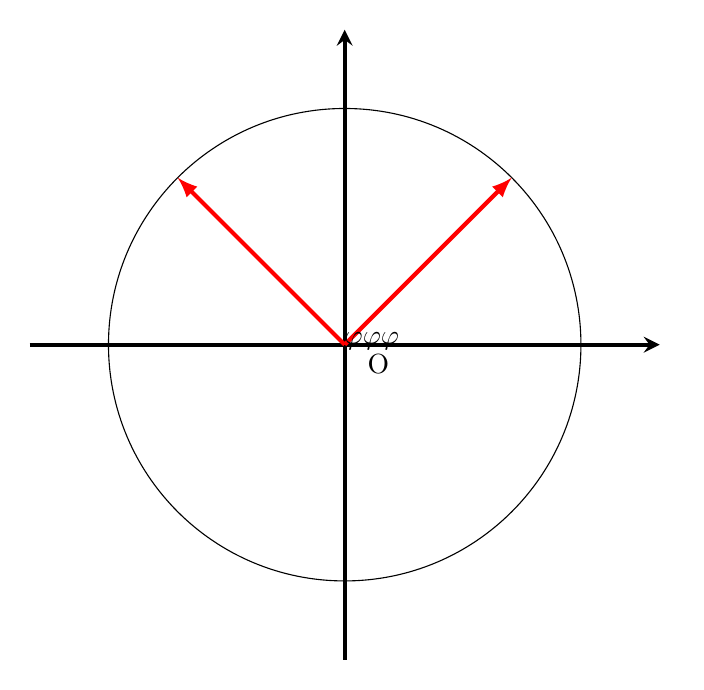
\begin{tikzpicture}
			\coordinate (O) at (0,0);
			\coordinate (v) at (4,0);
			\coordinate (A) at (45:3);
			\coordinate (B) at (90:3);
			\coordinate (C) at (135:3);
			\draw (O) circle[radius=3, line width=1.5pt];
			\draw[-stealth, line width=1.5pt] (-4,0)--(v);
			\draw[-stealth, line width=1.5pt] (0,-4)--(0,4);
			\draw[-latex, line width=1.5pt, red] (O)--(A);
			\draw[-latex, line width=1.5pt, red] (O)--(C);
			\tkzMarkAngle[size=0.75cm,color=blue,line width=1.0pt](v,O,A);
			\tkzLabelAngle[color=black,pos=1.2](v,O,A){$\varphi$};
			\tkzMarkAngle[size=0.85cm,color=blue,line width=1.0pt](A,O,B);
			\tkzLabelAngle[color=black,pos=1.2](A,O,B){$\varphi$};
			\tkzMarkAngle[size=0.85cm,color=blue,line width=1.0pt](B,O,C);
			\tkzLabelAngle[color=black,pos=1.2](B,O,C){$\varphi$};
			\node[below left] at (O) {O};
			\node[above] at (v) {$v$};
		\end{tikzpicture}
	\end{center}
	Đặt $\varphi=\omega\Delta t$.\\
	$4\varphi=\pi\Rightarrow \varphi=\xsi{\dfrac{\pi}{4}}{\radian}.$\\
	Tại thời điểm $t_1$:
	$$v=v_{\text{max}}\cdot\cos\dfrac{\pi}{4}=v_{\text{max}}\cdot\dfrac{\sqrt{2}}{2}\Rightarrow W=2W_{\text{đ1}}=\SI{200}{\milli\joule}.$$
	Tần số góc dao động:
	$$\omega=\sqrt{\dfrac{2W}{mA^2}}=\xsi{2\pi}{\radian/\second}.$$
	Giá trị của $\Delta t$:
	$$\Delta t=\dfrac{\varphi}{\omega}=\SI{0.125}{\second}.$$
		}
\end{ex}

\Closesolutionfile{ans}
\section{Câu trắc nghiệm đúng/sai} 
\textit{Thí sinh trả lời từ câu 1 đến câu 4. Trong mỗi ý \textbf{a)}, \textbf{b)}, \textbf{c)}, \textbf{d)} ở mỗi câu, thí sinh chọn đúng hoặc sai}
\setcounter{ex}{0}
\Opensolutionfile{ans}[ans/G11-4-TF]
% ===================================================================
\begin{ex}
	Cho các phát biểu dưới đây. Phát biểu nào là phát biểu đúng, phát biểu nào sai?
	\choiceTF[t]
	{\True Dao động điều hòa là dao động có li độ biến thiên theo thời gian theo qui luật hàm sin hoặc cosin}
	{\True Chu kì là khoảng thời gian ngắn nhất mà trạng thái dao động của vật được lặp lại như cũ}
	{Một vật dao động tuần hoàn thì chắc chắn dao động điều hòa}
	{Cơ năng của vật dao động điều hòa biến thiên tuần hoàn theo thời gian}
	\loigiai{}
\end{ex}
% ===================================================================
\begin{ex}
	Một vật nhỏ có khối lượng $\SI{100}{\gram}$ dao động điều hòa với phương trình $x=\xsi{4\cos\left(5\pi t+\dfrac{\pi}{3}\right)}{\centi\meter}$, $t$ được tính bằng giây. Lấy $\pi^2\approx10$.
	\choiceTF[t]
	{\True Chu kì dao động của vật là $\SI{0.4}{\second}$}
	{Tốc độ cực đại của vật là  $\xsi{20\sqrt{10}}{\meter/\second}$}
	{\True Năng lượng dao động của vật là $\SI{0.02}{\joule}$}
	{Trong khoảng thời gian $t =\SI{1.2}{\second}$, vật đi được quãng đường $\SI{12}{\centi\meter}$}
	\loigiai{}
\end{ex}
% ===================================================================
\begin{ex}
	Vật nhỏ dao động điều hòa trên trục $Ox$, vật đi từ biên này đến biên kia mất $\SI{0.157}{\second}$; khoảng cách giữa hai biên là $\SI{10}{\centi\meter}$. Lấy $\pi=3,14$.
	\choiceTF[t]
	{Chu kì dao động của vật là $\SI{0.157}{\second}$}
	{\True Vật thực hiện được 10 dao động trong $\SI{3.14}{\second}$}
	{\True Thời gian ngắn nhất vật đi từ vị trí $x =\SI{5}{\centi\meter}$ đến $x =\SI{-2.5}{\centi\meter}$ là $\SI{0.105}{\second}$}
	{\True Tốc độ của vật khi qua vị trí cân bằng là $\SI{1}{\meter/\second}$}
	\loigiai{}
\end{ex}
% ===================================================================
\begin{ex}
	Một vật dao động điều hòa có phương trình $x=\xsi{4\cos\left(2\pi t-\dfrac{\pi}{2}\right)}{\centi\meter}$. 
	\choiceTF[t]
	{Vật chuyển động trên quỹ đạo dài $\SI{4}{\centi\meter}$}
	{\True Phương trình vận tốc của vật có dạng là $v=\xsi{-8\pi\sin\left(2\pi t-\dfrac{\pi}{2}\right)}{\centi\meter/\second}$}
	{\True Tại vị trí $x=\pm\dfrac{A\sqrt{3}}{2}$  thì động năng bằng một phần ba thế năng}
	{\True Đồ thị tọa độ - thời gian của vật là hình dưới đây\\
	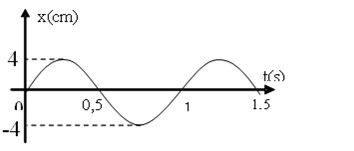
\includegraphics[width=0.4\linewidth]{../figs/D11-004-3}
	}
	\loigiai{}
\end{ex}

\Closesolutionfile{ans}
\section{Câu trắc nghiệm trả lời ngắn} \textit{Thí sinh trả lời từ câu 1 đến câu 6}
\setcounter{ex}{0}
\Opensolutionfile{ans}[ans/G11-4-TL]
% ===============================================================
\begin{ex}
	Một vật có khối lượng $m =\SI{2}{\kilogram}$ dao động điều hòa theo phương trình $x=\xsi{10\cos\left(\dfrac{2\pi}{3}\cdot t+\pi\right)}{\centi\meter}$. Lấy $\pi^2=10$. Động năng của vật tại thời điểm $t=\SI{15.5}{\second}$ là bao nhiêu? \textit{(Tính theo đơn vị joule ($\si{\joule}$) và làm tròn đến 2 chữ số sau dấu phẩy thập phân)}. 
	\shortans{0,03 }
	\loigiai{
		Phương trình vận tốc $v=\xsi{-\dfrac{20\pi}{3}\sin\left(\dfrac{2\pi}{3}\cdot t+\pi\right)}{\centi\meter/\second}$.\\
		Tại thời điểm $t=\SI{15.5}{\second}\Rightarrow v\approx\SI{18.14}{\centi\meter/\second}$.\\
		Động năng của vật tại thời điểm đó:
		$$v=\dfrac{1}{2}mv^2\approx\SI{0.03}{\joule}$$
	}
\end{ex}
% ===============================================================
\begin{ex}
	Một vật nhỏ dao động điều hòa dọc theo trục $Ox$. Khi vật cách vị trí cân bằng một đoạn $\SI{2}{\centi\meter}$ thì động năng của vật là $\SI{0.48}{\joule}$. Khi vật cách vị trí cân bằng một đoạn $\SI{6}{\centi\meter}$ thì động năng của vật là $\SI{0.32}{\joule}$. Biên độ dao động của vật bằng bao nhiêu \textit{(tính theo đơn vị $\si{\centi\meter}$ và làm tròn đến 1 chữ số thập phân)}. 
	\shortans{10}
	\loigiai{
		$$\begin{cases}
			\frac{1}{2}m\omega^2\left(A^2-x^2_1\right)=\SI{0.48}{\joule}\\
			\frac{1}{2}m\omega^2\left(A^2-x^2_2\right)=\SI{0.32}{\joule}
		\end{cases}\Rightarrow \dfrac{A^2-2^2}{A^2-6^2}=\dfrac{0,48}{0,32}\Rightarrow A=\SI{10}{\centi\meter}.$$
	}
\end{ex}
% ===============================================================
\begin{ex}
	Một con lắc lò xo gồm vật nhỏ có khối lượng $\SI{270}{\gram}$ và lò xo nhẹ độ cứng $\SI{30}{\newton/\meter}$ dao động điều hòa trên phương nằm ngang với biên độ $\SI{8}{\centi\meter}$. Chọn mốc thời gian $(t = 0)$ lúc vật đi qua vị trí có li độ $\SI{4}{\centi\meter}$ và hướng về vị trí cân bằng. Lấy $\pi^2=10$. Sau bao lâu kể từ lúc $t = 0$, vật có li độ cực đại lần đầu tiên? \textit{(Kết quả tính theo $\si{\second}$)}.
	\shortans{0,5 }
	\loigiai{
		$$\Delta t=\dfrac{5}{6}T=\dfrac{5}{6}\cdot 2\pi\sqrt{\dfrac{m}{k}}=\SI{0.5}{\second}.$$
	}
\end{ex}
% ===============================================================
\begin{ex}
	Một vật dao động điều hòa, khi vật có vận tốc $v_1=\xsi{5\pi\sqrt{3}}{\centi\meter/\second}$  thì gia tốc của vật là $a_1=\xsi{-5\pi^2}{\centi\meter/\second^2}$. Khi vật có vận tốc $v_2=\xsi{-5\pi\sqrt{2}}{\centi\meter/\second}$  thì gia tốc của vật là $a_2=\xsi{5\pi^2\sqrt{2}}{\centi\meter/\second^2}$. Lấy $\pi^2=10$. Tính tần số của dao động của vật theo đơn vị hertz.
	\shortans{0,5}
	\loigiai{
		$$\dfrac{v^2_1}{\omega^2}+\dfrac{a^2_1}{\omega^4}=\dfrac{v^2_2}{\omega^2}+\dfrac{a^2_2}{\omega^4}\Rightarrow \omega=\xsi{\sqrt{10}}{\radian/\second}$$
		Tần số dao động của vật:
		$$f=\dfrac{\omega}{2\pi}=\SI{0.5}{\hertz}.$$
	}
\end{ex}
% ===============================================================
\begin{ex}
	Hai dao động được mô tả như hình vẽ. Lấy $\pi=3,14$. Độ lệch pha giữa hai dao động này bằng bao nhiêu? \textit{(Kết quả làm tròn đến 2 chữ số sau dấu phẩy thập phân)}. 
	\begin{center}
		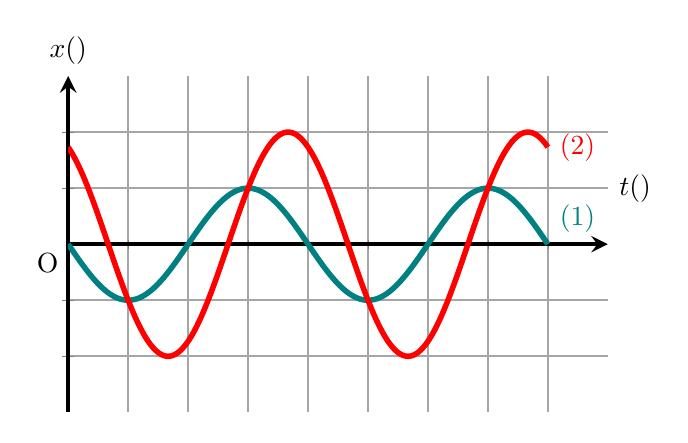
\begin{tikzpicture}  
			\begin{axis}[  ultra thick,yscale=0.75,
				xmin=0,  
				xmax=9,  
				xtick={0,1,...,8},
				ytick={-2,-1,...,2},
				minor x tick num=0,
				minor y tick num=0,
				ymin=-3,  
				ymax=3, 
				samples=300,
				yticklabels=\empty,
				xticklabels=\empty,
				axis lines=center, 
				grid style={step=1, line width =0.4pt, color=gray!40!white},
				grid=both, %giới hạn ô lưới
				major grid style={line width=0.75pt,gray!70!white},
				xlabel=$\xsi{t}{\left(\si{\second}\right)}$, 		ylabel=$\xsi{x}{\left(\si{\centi\meter}\right)}$,
				every axis y label/.style={at=(current axis.above origin),anchor=south},  
				every axis x label/.style={at=(current axis.right of origin),anchor=west},  ]
				\addplot [line width=2pt, teal, smooth, domain=0:8] {1*cos(deg(pi*x/2+pi/2))} node[above right] {$(1)$}; 
				\addplot [line width=2pt, red, smooth, domain=0:8] {2*cos(deg(pi*x/2+pi/6))} node[right] {$(2)$}; 
				\coordinate (O) at (axis cs: 0,0);
			\end{axis}  
			\node[below left] at (O) {O};
		\end{tikzpicture}
	\end{center}
	\shortans{1,05}
	\loigiai{
		Tại thời điểm vật (1) qua vị trí biên dương thì vật 2 qua vị trí $x=\dfrac{A}{2}$ theo chiều dương $\Rightarrow \Delta\varphi=\xsi{\dfrac{\pi}{3}}{\radian}.$
	}
\end{ex}
% ===============================================================
\begin{ex}
	Một chất điểm dao động điều hòa dọc theo trục $Ox$ với tần số $\SI{1}{\hertz}$, cơ năng bằng $W$. Hình bên là đồ thị biểu diễn sự thay đổi của động năng $W_{\text{đ}}$ theo thế năng $W_{\mathrm{t}}$ của một chất điểm. 
	\begin{center}
		\begin{tikzpicture}  
			\begin{axis}[  ultra thick,scale=0.75,
				xmin=0,  
				xmax=7,  
				ytick={0,1,...,4},
				minor y tick num=0,
				ymin=0,  
				ymax=5, 
				samples=300,
				yticklabels=\empty,
				xticklabels=\empty,
				xtick=\empty,
				axis lines=center, 
				grid style={step=1, line width =0.4pt, color=gray!40!white},
				grid=both, %giới hạn ô lưới
				major grid style={line width=0.8pt,gray!75!white},
				xlabel=$W_{\text{t}}$, 		ylabel=$W_{\text{đ}}$,
				every axis y label/.style={at=(current axis.above origin),anchor=south},  
				every axis x label/.style={at=(current axis.right of origin),anchor=west},  ]
				\addplot [line width=2pt, blue, smooth, domain=0:6] {4-4*x/6};  
				\coordinate (O) at (axis cs: 0,0);
				\fill   (axis cs: 1.5,3) circle[radius=2pt]  node [above right] {M};
				\fill   (axis cs: 4.5,1) circle[radius=2pt]  node [above right] {N};
			\end{axis}  
			\node[below left] at (O) {O};
		\end{tikzpicture}
	\end{center}
	Ở thời điểm $t$ nào đó, trạng thái năng lượng của vật có vị trí M như trên đồ thị, lúc này chất điểm đang ở li độ $x =\SI{2}{\centi\meter}$. Khi vật có trạng thái năng lượng ở vị trí N trên đồ thị thì tốc độ của vật bằng bao nhiêu $\si{\centi\meter/\second}$. Lấy $\pi^2=10$. \textit{(Kết quả làm tròn đến 3 chữ số có nghĩa)}. 
	\shortans{12,6}
	\loigiai{
		Tại M:
		$$W_{\text{đM}}=\dfrac{3}{4}W\Rightarrow W_{\mathrm{t}}=\dfrac{1}{4}W\Rightarrow A=2x=\SI{4}{\centi\meter}.$$
		Tại N:
		$$W_{\text{đN}}=\dfrac{1}{4}W\Rightarrow v_{\mathrm{N}}=\dfrac{1}{2}\omega A\approx\SI{12.6}{\centi\meter/\second}.$$
	}
\end{ex}
\Closesolutionfile{ans}
\begin{center}
	\textbf{--- HẾT ---}
\end{center}